\documentclass{article}
\usepackage[letterpaper,top=2cm,bottom=2cm,left=3cm,right=3cm,marginparwidth=1.75cm]{geometry}

% === Useful packages ===
\usepackage[german]{babel}
\usepackage[letterpaper,top=2cm,bottom=2cm,left=3cm,right=3cm,marginparwidth=1.75cm]{geometry}

\parindent 0px % remove Paragraph indentation

\usepackage{amsmath, amssymb, amsfonts}
\usepackage{graphicx}
% \usepackage{float}

% \usepackage[colorlinks=true, allcolors=blue]{hyperref}
\usepackage{xcolor}

% --- manage multicols ---
\usepackage{multicol}
\usepackage{paracol} % cause multicol does not work properly over several pages I have to use paracol
\setcolumnwidth{0.30\textwidth}
\setlength\columnsep{20pt}  
\setlength{\columnseprule}{0.5pt}

\title{Signal und System Theorie  \\ [1ex] \large Fachsemester 3}
\author{Prof. Dr.-Ing. Frank Giesecke}
\date{}

\begin{document}
\maketitle

\newpage
\tableofcontents

\newpage
\section{\centering Literatur}
\begin{table}[!ht]
	\centering
	\begin{tabular}{|l|l|}
		\hline
		Title & Author \\
		\hline\hline
		Signal und Systemtheorie & Frey Bassardi \\
		\hline
		Grundlagen der Informationstechnik & Martin Meyer \\
		\hline
		Angewandte Systemtheorie. Kontinuierliche und zeitdiskrete Signalverarbeitung & Dieter Kreß, Ralf Irmer \\
		\hline
		Signal- und Systemtheorie in Beispielen & Eberhard Voigt \\
		\hline
	\end{tabular}
\end{table}


\newpage
\section{\centering 16.10.2024 (ohne Grafiken)}
\subsection{System}
\begin{figure}[!ht]
	\centering
	\includegraphics[width=3cm]{example-image}
	\caption{System}\label{Abb. System}
\end{figure}

\subsection{Teilsystem}
\begin{figure}[!ht]
	\centering
	\includegraphics[width=3cm]{example-image}
	\caption{Teilsystem}\label{Abb. Teilsystem}
\end{figure}

\subsection{Beispiel: RC-Tiefpass}
\begin{figure}[!ht]
	\centering
	\includegraphics[width=3cm]{example-image}
	\caption{RC-Tiefpass}\label{Abb. RC-Tiefpass}
\end{figure}

\subsection{Regelkreis}
\begin{figure}[!ht]
	\centering
	\includegraphics[width=3cm]{example-image}
	\caption{Regelkreis}\label{Abb. Regelkreis}
\end{figure}

\columnratio{0.5}
\begin{paracol}{2}
	{\large Analogsignal (kontinuirlich)}
	\begin{figure}[!ht]
		\centering
		\includegraphics[width=3cm]{example-image}
		\caption{kontinuierliches Signal}\label{Abb. kontinuierliches Signal}
	\end{figure}
	Zu jedem Zeitpunkt ein beliebig definierter Wert.
	\switchcolumn
	Digitalsignal (diskret)
	\begin{figure}[!ht]
		\centering
		\includegraphics[width=3cm]{example-image}
		\caption{diskretes Signal}\label{Abb. diskretes Signal}
	\end{figure}
\end{paracol}

\subsection{Signalbeschreibung}
\columnratio{0.5}
\begin{paracol}{2}
	{\large Leistungssignale} \\
	Zeitlich unbegrenzter Verlauf \\
	(auch einseitig unendlich)
	\begin{figure}[!ht]
		\centering
		\includegraphics[width=3cm]{example-image}
		\caption{Leistungssignal}\label{Abb. Leistungssignal}
	\end{figure}
	\switchcolumn
	{\large Energiesignale} \\
	Zeitlich Begrenzt
	\begin{figure}[!ht]
		\centering
		\includegraphics[width=3cm]{example-image}
		\caption{Energiesignal}\label{Abb. Energiesignal}
	\end{figure}
\end{paracol}


\newpage
\section*{\centering 21.10.2024 (Vorlesung noch nicht nachgetragen)}
\section*{\centering 23.10.2024 (Vorlesung noch nicht nachgetragen)}


\newpage
\section*{\centering 28.10.2024}
\subsection*{Wiederholung}
\begin{enumerate}
	\item Leistungssignale \\
	Gleichanteil/ linearer Mittelwert/ Moment 1. Ordnung \\
	$\Bar{x} = (coming_soon)$
	\[ f(x) = \lim_{T\to\infty} \int_{-T}^{T} x^2 \,dt \]

	\item Signalgleichleistung \\
	(Leistung, die den Gleichanteil verursacht) \\
	$P_{x=} = \Bar{x}^2 = m_1^2$

	\item mittlere Signalleistung/ quadratische Mittelwert/ Gesamt-Signalleistung / Moment 2. Ordnung \\
	$P = \Bar{x^2} = m_2 = (coming_soon)$

	\item Effektivwert (Wurzel aus der mittleren Signalleistung) \\
	$x_{eff}=\sqrt{P}=\sqrt{x^2}$

	\item Signalwechselleistung/ Varianz/ Zentral-Moment 2. Ordnung \\
	$P_{x~}=\sigma^2 = \mu_2 = P_x - P_{x=} = \Bar{x^2} - \Bar{x}^2$

	\item Standartabweichung \\
	$\sigma = \sqrt{P_{x~}} = \sqrt{\mu_2}$
\end{enumerate}

\subsection*{Alternative Berechnung der Signalwechselleistung/ Varianz/ Zentral-Moment 2. Ordnung}
$P_{x~} = (coming_soon)$ \\
$P_{x~} = P_x - P_x$

\subsection*{Direkte Berechnung der Varianz/ Signalwechselspannung aus einem Datensatz (digital)}
\paragraph{Fallunterscheidung}
\columnratio{0.5}
\begin{paracol}{2}
    linerer Mittelwert/ Gleichanteil ist bekannt oder kann exakt bestimmt werden. \\
    $\Bar{x} ist bekannt$ \\
    $\sigma^2 = P_{x~} = \mu_2 = (coming_soon)$
    
    \switchcolumn
    linearer Mittelwert wird aus den N Werten bestimmt. \\
    $\Bar{x} ist un-bekannt$ \\
    $\Bar{x_N} = (coming_soon)$ \\
    $\sigma^2 = P_x = (coming_soon)$
\end{paracol}
\begin{center} N = Anzahl der Werte \end{center}

\subsection*{Es folgt:}
Angenäherter Einheitssprung, Einheitssprung-Funktion, Einheitsimpuls-Funktion, Deltaimpuls/ Dirac-Impuls, Einheitsanstiegs-Funktion

\subsection*{Angenäherter Einheitssprung ($\delta$ delta)}
\columnratio{0.3}
\begin{paracol}{3}
	(grafic is coming soon)

	\switchcolumn
	\begin{center}
    	$\overrightarrow{Differentation}$ \\
		$(\frac{d}{dt})$ \\
		\vspace{1em}
		$\overleftarrow{Integration}$ \\
		$\hookrightarrow$ Intigrationsgrenzen \\
		$-\infty bis aktueller Zeitpunkt (t)$ \\
		$\sigma = (coming_soon)$
	\end{center}

	\switchcolumn
	(grafic is coming soon)
\end{paracol}

\newpage
\section*{\centering 30.10.2024 (Vorlesung noch nicht nachgetragen)}
\section*{\centering 06.11.2024 (Vorlesung noch nicht nachgetragen)}
\section*{\centering 04.11.2024 (Vorlesung noch nicht nachgetragen)}


\newpage
\section*{\centering 11.11.2024}
\subsection*{Ergänzung: Kreuzrelation}

\[
	E_{x1x2}(\tau)=\int_{-\infty}^{\infty}x(t)*x_2(t+\tau)*dt 
\]
mindestens eines der Verläufe muss ein Energiesignal sein. \\
Wenn beide Verläufe $x_1$ und $x_2$ Leistungssignale sind, dann:
\[
	Allg. Variante: P_{x1x2}(\tau)=\lim_{T\to\infty}x_1(t)x_2*x_2(t+\tau)*dt
\]
bei Vorliegen einer Periodizität von $x_1$ und $x_2$
\[
	P_{x1x2}(\tau)=\frac{1}{T}\int_{0}^{T}x(t)*x_2(t+\tau)*dt
\]
entweder T als gleiche Periode bei den Verläufen oder T als gemeinsames Vielfaches der beiden Periodenduaer von $x_1$ und $x_2$

\subsection*{Das System}
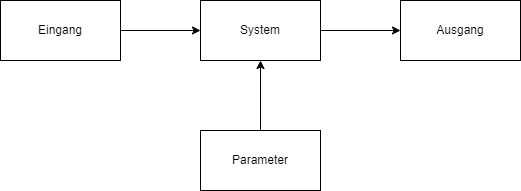
\includegraphics[scale=0.8]{img/2024_11_11.png}

\subsubsection*{Im Zeitbereich:}
z.B. Spannung $u_e(t) \to u_a(t)$ \\
oder digital/zeitdiskret

\subsubsection*{System im Laplace Bereich}
$s=\sigma+j\omega$ \\
(system im laplace-bereich bild fehlt wurde aber schon erstellt)

\subsubsection*{System in Frequenzbereich}

\subsubsection*{System-Eigenschaften}
4 Grundeigenschaften:
\begin{itemize}
    \item Linearität
    \begin{itemize}
        \item linear
        \item licht linear
    \end{itemize}
    
    \item Zeitinvarianz
    \begin{itemize}
        \item Zeit-konstant
        \item Zeit-veränderlich
    \end{itemize}
    
    \item Kausalität
    \begin{itemize}
        \item kausal
        \begin{itemize}
            \item statisch (speicherlos)
            \item dynamisch (mit Speicherelementen)
        \end{itemize}
        \item a-kausal (nicht kausal)
    \end{itemize}
    
    \item Stabilität
    \begin{itemize}
        \item Stabil
        \item Grenz-Stabil
        \item In-Stabil
    \end{itemize}
\end{itemize}


\newpage
\section*{13.11.2024 (fehlt)}
war krank und muss noch nachtragen


\newpage
\section*{\centering 18.11.2024 (Bilder fehlen)}
die Aufzeichnung dieser Stunde habe ich auf dem Papier gemacht und muss noch nachgetragen werden.
\subsection*{Stabilität von Systemen}
\begin{paracol}{3}
	{\large Stabil}
	\begin{itemize}
		\item \textcolor{red}{BIBO-Stabilität} (Bounded Input - Bounded Output) $\to$ \textcolor{red}{Amplitudenstabilität}
		\item Nachweis via Beträgsfläche
		\begin{center}
			$\int_{-\infty}^{\infty}|g(t)| < \infty \rightarrow stabil$
		\end{center}
		(äquivalent mit der Summe für zeitdiskrete Systeme)
	\end{itemize}

\switchcolumn
	{\large Grenzstabil}
	\begin{itemize}
		\item Anwendung: \\
		Analoger Funktionsgenerator
	\end{itemize}

\switchcolumn
	{\large Instabil} \\
	Amplitude gegen $\infty$
\end{paracol}

\paragraph{Klassifizierung} über das praktische Stromverhalten \\
\begin{paracol}{3}
	(Ilustration Eingangssignal $\to$ Ausgangssignal (gegen 0))

	\switchcolumn
	(Ilustration Eingangssignal $\to$ Ausgangssignal (konstante))

	\switchcolumn
	(Ilustration Eingangssignal $\to$ Ausgangssignal (gegen unendlich))
\end{paracol}

\paragraph{Mathematisch} über Laplace $\&$ z-Transformation
\begin{center}
	zeit-kontinuirlich / Laplace-Transformation:  $g(t) \rightarrow G(s) = \frac{Zaehler(s)}{Nenner(s)}$ \\
	zeit-diskret / t-Transformation: $g(k) \rightarrow G(Z) = \frac{Zaehler(z)}{Nenner(z)}$
\end{center}
Nullsetzten des Zaehlers $\rightarrow$ Nullstellen der Übertragungsfunktion \\
Nullsetzten des Nenners $\rightarrow$ Polstellen der Übertragungsfunktion
\begin{center} (folgt in der nächsten Vorlesung) \end{center}

\newpage
\section*{\centering 20.11.2024}
\subsection*{Stabilitätsbestimmung über die Übertragungsfunktion}
\begin{itemize}
	\item analoge/zeitkontinuierliche Systeme $G(s)$ Übertragungsfunktion \\
	s: Laplace Variable \\
	$s=\delta+j\omega$
	\item digitale/zeitdiskrete Systeme $G(z)$ Übertragungsfunktion \\
	z: z-Variable \\
	$z=Re(z) + j * Im(z) = |z| * e^{j*\phi_z} $
\end{itemize}
Nullsetzen des ZählerTerms $(G(s) bzw. G(z))$ liefert die Nullstellen \\
Nullsetzen des Nenner-Terms $(G(s) bzw. G(z))$ liefert die Polstelle \\
Wenn eine Nullstelle nicht genau auf eine Polstelle fällt haben die Nullstellen keinen Einfluss auf die Stabilität. \\
Wenn eine Nullstelle genau auf eine Polstelle fällt, wird die entsprechende Polstelle ausgelöscht.
\begin{center}
Bsp.:
\[
G(s) = \frac{ (s-s_{01}) * (s-s_{0n}) }{ (s-s_{p1}) * (s-s_{pn}) }*K
\]
\end{center}

\subsubsection*{Betrachtung der verbleibenden (nicht durch Nullstellen ausgelöschten) Polstellen zur Stabilitätsbestimmung}
Betrachtung der Lage der Polstellen in den Ebenen
\columnratio{0.5}
\begin{paracol}{2}
$G(s) \rightarrow$  s-Ebene \\
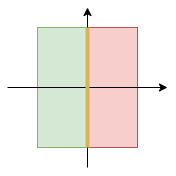
\includegraphics[scale=0.8]{img/2024_11_20_s-Ebene.png}
\begin{itemize}
	\item Polstellen link von der $j\omega$-Achse \\
	$\rightarrow$ System ist Stabil
	\item mindestens eine Polstelle rechts der $j\omega$-Achse oder mindestens eine mehrfache Polstelle auf der $j\omega$-Achse \\
	$\rightarrow$ System ist stabil
	\item keine Posstelle rechts der $j\omega$-Achse und nur einfache Polstellen (beliebiger Anzahl an unterschiedlichen Stellen) \\
	$\rightarrow$ System ist grenzstabil
\end{itemize}
\paragraph{Bsp. Integrator}
\[
E \rightarrow G_I(s)=\frac{1}{s} = s^{-1} \rightarrow A
\]
2 Intigratoren in Kette:
\[
E \rightarrow s^{-1} \rightarrow s^{-1} \rightarrow A
\]
$\rightarrow$ 2 grenzstabile Systeme werden zusammen 1 instabiles System

\switchcolumn

$G(z) \rightarrow$ z-Ebene \\
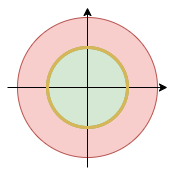
\includegraphics[scale=0.8]{img/2024_11_20_z-Ebene.png}
\begin{itemize}
	\item alle Polstellen innerhalb des Einheitskreises (nicht auf dem Einheitskreis) \\
	$\rightarrow$ System ist stabil
	\item mindestens eine Polstelle außerhalb des Einheitskreises oder mindestens eine mehrfache Polstelle auf dem Einheitskreis \\
	$\rightarrow$ System ist stabil
	\item keine Polstelle außerhalb des Einheitskreises und nur einfache Polstellen (beliebiger Anzahl an unterschiedlichen Stellen) auf dem Einheitskreis \\
	$\rightarrow$ System ist grenzstabil
\end{itemize}
\paragraph{Bsp. Integrator}
\[
E \rightarrow s^{-1} \rightarrow s^{-1} \rightarrow A
\]
\[
G_{ges} = G_1(s) * G_2(s) = s^{-2}
\]
doppelte Polstelle bei 0 \\
$\rightarrow$ 2 stabile Systeme werden zusammen 1 instabiles System
\end{paracol}


\newpage
\section*{\centering 25.11.2024}
\subsection*{Anforderung an die Systemeigenschaften zur Anwendbarkeit von Werkzeugen der Systemtheorie}
Beschreibung eines Systems durch:
\begin{itemize}
	\item Impulsantwort: $g(t), g(k)$; Sprungantwort: $h(t), h(k)$; Anstiegsanwort: $a(t), a(k)$ \\
	System muss linear und zeitinvariant sein. \\
	(Kausalität und Stabilität sind beliebig)
	\begin{center}
		$h(t) = \int_{0}^{t}g(t)*d\tau$ \\
		$g(t) = \frac{dh(t)}{dt}$
	\end{center}
	
	\item Übertragungsfunktion: $G<(s)$ (Laplace), $G(z)$ (z-Transformation) \\
	System muss linear, zeitinvariant und kausal sein. \\
	(Stabilität spielt keine Rolle)

	\item Komplexer Frequenzgang $G(j\omega)$, $G(\omega)$, G(jf), G(f) bzw. G(m) \\
	System muss linear, zeitinvariant und stabil oder grenzstabil sein. \\
	(Kausalietät spielt keine Rolle)
	\begin{center}
		Fourier-Transformation: $g(t) \rightarrow G(j\omega)$ \\
		Diskrete-Fourier-Transformation: $g(t) \rightarrow G(m)$
	\end{center}
\end{itemize}

\paragraph{Querverbindung:}
$G(s) \rightarrow G(j\omega)$, $G(\omega)$,  G(jf) oder G(f) \\
$s=\delta + j\omega \rightarrow \delta = 0$\\
Nur bei einem stabilen oder Grenzstabilen System erlaubt.

\subsection*{Ausgang eines linearen und zeitinvarianten Systems zur System-Charakterisierung}
\paragraph{Deltaimpuls} ist am besten geeignet weil: 
\begin{itemize}
	\item besitzt alle Frequenzanteile
	\item alle Frequenzanteile haben die selbe Intensität
\end{itemize}
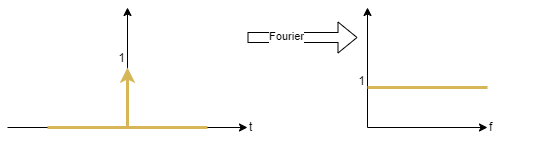
\includegraphics[scale=0.8]{img/2024_11_25_fourier_deltaimpuls.png}

\paragraph{Einheitssprung:} \mbox{} \\
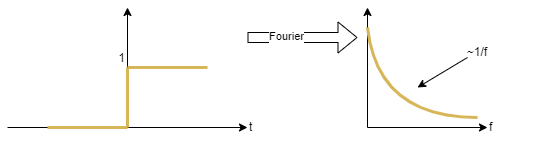
\includegraphics[scale=0.8]{img/2024_11_25_fourier_einheitssprung.png}

\paragraph{Einheitsanstieg:} \mbox{} \\
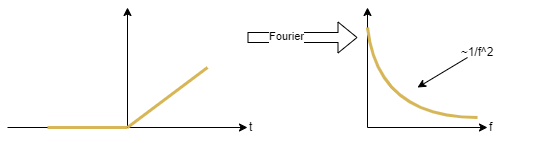
\includegraphics[scale=0.8]{img/2024_11_25_fourier_einheitsanstieg.png}

\subsection*{Ermittlung des Ausgangssignals aus einem Eingangssignal bei bekannter Impulsantwort g(t) bzw. g(k)}
Eingangssignal x(t) $\rightarrow$ System g(t) $\rightarrow$ Ausgangssignal y(t)

\paragraph{Faltungsoperation (*):}
\begin{center}
$ y(t) = x(t) * g(t)$ \\
(Faltung wird durch Transformation zur komplexen Multiplikation) \\
\mbox{} \\
$y(t) = x(t) * g(t) = \int_{-\infty}^{\infty} x(t) \cdot g(-\tau + t) d\tau$ \\
(äquivalent mit Summe für zeitdiskrete Systeme)
\end{center}

\paragraph{Kreuzkorrelation (schon mal gemacht)}
\begin{center}
$E_{x_1x_2}(\tau) = \int_{-\infty}^{\infty} x_1(t) * x_2(t + \tau) * dt$ \\
(Im prinzip das selbe wie die Faltungsoperation nur mit einer anderen Intention)
\end{center}


\newpage
\section*{\centering 27.11.2024}
\begin{center}
	x(t) $\to$ System mit Impulsantwort g(t) $\to$ y(t) \\ \mbox{} \\
	$y(t) = x(t) * g(t)$ \\ \mbox{} \\
	$y(t) = \int_{-\infty}^{\infty} x(\tau) \cdot g(-\tau + t) \cdot d\tau = \int_{-\infty}^{\infty} x(-\tau +t) \cdot g(\tau) \cdot d\tau $ 
\end{center}
\subsubsection*{Beispiel Faltung}
$u_e(t) \to g(t) \to u_a(t)$ \\
\columnratio{0.5}
\begin{paracol}{2}
	$u_e(t)$ \\
	$u_e(t) = 2V \cdot rect(\frac{t-3s}{4s})$ \\
	(Grafic fehlt)
	\switchcolumn
	$g(t)$ \\
	$g(t) = 0.5s^{-1} \cdot rect(\frac{t-1s}{2s})$ \\
	(Grafic fehlt)
\end{paracol}
\mbox{} \\
neue Variable für die Zeitachse weil t Verschiebeparameter wird \\
$t \to \tau$

\subsubsection*{Spiegelung einer Funktion}
Gespiegelte Funktion über $\tau$ wird um t verschoben: Verschiebe-Richtung wird ebenfalls gespiegelt

\subsubsection*{Zeitliches Übereinanderlegen der Funktion}
z.B. auf eine $\tau$-Achse \\
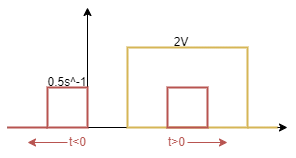
\includegraphics[width=0.6\textwidth]{img/2024_11_27_achsenverschiebung.png} \\
Funktion muss sich zeitlich überlagern damit $u_a(t) > 0V$ \\
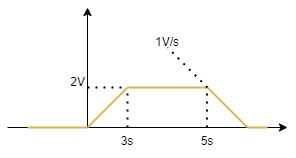
\includegraphics[width=0.6\textwidth]{img/2024_11_27_rect_multiplikation.png} \\
$u_a(1s < t < 3t) = \int_{1s}^{t+1s} 2V \cdot 0.5s^{-1} \cdot d\tau$

\subsection*{Kreuzkorrelation}
$E_{x1,x2}(\tau) = \int_{-\infty}^{\infty}\cdot x_2(t+\tau) \cdot t$ \\
\subsubsection*{Unterschiede zur Faltung}
\begin{itemize}
	\item keine Umbenennung der Achsen nötig, 
	\item keine Spiegelung erforderlich \\
	(aber: Änderung der Verschieberichtung durch das $\tau$)
\end{itemize}
\subsubsection*{Darstellung über einer Zeitachse}
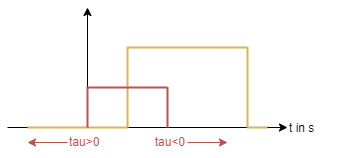
\includegraphics[width=0.6\textwidth]{img/2024_11_27_kreuzkorrelation.png} \\
$E_{u1,u2}(\tau = 0) = 2V \cdot 0.5V \cdot 1s = 1V^2s$ \\
$E_{u1,u2}(\tau >= 1s) = 0V$ \\
$E_{u1,u2}(\tau <= 5s) = 0V$ \\
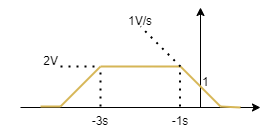
\includegraphics[width=0.6\textwidth]{img/2024_11_27_kreuzkorrelation_multiplikation.png}


\newpage
\section*{\centering 02.12.2024}
\subsection*{Transformationen auf Basis von Cos- und Sin}
(Was genau hat das Folgende mit Cos und Sin zu tun?)
\begin{center}
	\columnratio{0.5}
	\begin{paracol}{2}
		Laplace
		\switchcolumn
		Fourier
	\end{paracol}
	(Umkehrbar eindeutige Transformation)
	\paragraph{Transformations-Kerne} \mbox{} \\
	\columnratio{0.33}
	\begin{paracol}{3}
		$e^{-st}$ \\
		$e^{+st}$
		\switchcolumn
		Hintransformation \\
		Rücktransformation
		\switchcolumn
		$e^{-j\omega t}$ \\
		$e^{+j\omega t}$
	\end{paracol}	
\end{center}
\paragraph{Laplace Transformation} \mbox{} \\
transformiert werden 
\begin{itemize}
	\item Signale (allg. Terstsignale wie Einheitstsprung oder Delta-Inpuls)
	\item Beschreibung von Systemen (allg. die Impulsantwort)
\end{itemize}
\[ X(s) = \int_{0}^{+\infty} x(t) \cdot e^{-st} \cdot dt \]
\paragraph{Fourier Transformation} \mbox{} \\
transformiert werden
\begin{itemize}
	\item Signale (jeder mögliche Verlauf mit dem Ziel des Erhalts der Frequenzanteile des Signals)
	\item Beschreibung von Systemen (im Allgemeinen die Impulsantwort zum Erhalt des komplexen Frequenzgangs)
\end{itemize}
\[ X(j\omega) = \int_{-\infty}^{+\infty} x(t) \cdot e^{-j\omega t} \cdot dt \]

\columnratio{0.5}
\begin{paracol}{2}
	\paragraph{Laplace} \mbox{} \\
	Paramerter s:
	\begin{itemize}
		\item komplexe
		\item $s = \delta + j\omega$
	\end{itemize}
	Anwendung: \\
	Erkennung der Stabilität \\
	Problem: bei instabielen Systemen Impulsantwort steigt bis ins Unendliche an Ansteigen wird kompensiert durch den Faktor $e^{-st}$ mit $\delta > 0$
	\switchcolumn
	\paragraph{Fourier} \mbox{} \\
	Paramerter $j \omega$:
	\begin{itemize}
		\item rein imaginär
	\end{itemize}
	Anwendung: \\
	Faltung zu multiplikationen Auslösen \\
	(Reihen- /Kettenschaltung von Systemen)
	\[ g_{ges}(t) = g_1(t) * g_2(t) \]
\end{paracol}

\paragraph{Anwendung in Rückgekoppelten Systemen} \mbox{} \\
(Grafik \& Herleitung fehlt)
\[ G_{ges}(s) = \frac{X_a(s)}{X_e(s)} = \frac{G_1(s)}{1+ G_1(s) \cdot G_2(s)} \]

\paragraph{Anwendung der Labplace Transformation} \mbox{} \\
Auslösung von Integration und Differentation mit der Laplace-Transformation \\
\[ y(t) = \int_{0}^{t} x(\tau) \cdot d\tau \to y(s) = X(s) \cdot \frac{1}{s} \]
\[ y(t) = \frac{dx(t)}{dt} \to y(s) = X(s) \cdot s \]


\newpage
\section*{**.12.2024}


\end{document}














